\subsection{Lightcurve}\label{ssec:lightcurve}

Time series data and their analysis are a fundamental aspect of solar
physics for which many data sources are available.
SunPy provides a \texttt{LightCurve} class
with a convenient and consistent interface for handling solar time-series
data.  The main engine behind the \texttt{LightCurve} class is
the \href{http://pandas.pydata.org}{\texttt{pandas}} data-analysis library, and 
\texttt{LightCurve}'s \texttt{.data} attribute is a \texttt{pandas.DataFrame} 
class.
The \texttt{pandas} library contains a large amount
of functionality for manipulating and analysing time-series data,
making it an ideal basis for \texttt{LightCurve}.  \texttt{LightCurve}
assumes that the input data are time-ordered list(s) of numbers, and each
list becomes a column in the \texttt{pandas} DataFrame class.

Currently, the \texttt{LightCurve} class is compatible with the
following data sources: the GOES X-ray Sensor (XRS), PROBA2/LYRA, and
the SDO EUV Variability Experiment (EVE; only the level ``OCS'' and
% Do we need to explain what OCS means?
average CSV files -- see \url{http://lasp.colorado.edu/home/eve/data/}
for more detail).  For each of these instruments, a subclass of the
\texttt{LightCurve} object is initialised
(\textit{e.g.}, \texttt{GOESLightCurve}) which inherits from
\texttt{LightCurve} but allows instrument-specific functionality to be
included.  Future developments will introduce support for additional
instruments and data products, as well as implementing a factory interface 
similar to that of \texttt{Map}.  Since there is no established standard
as to how time-series data should be stored and distributed, each SunPy 
\texttt{LightCurve} object sub-class provides the ability to download its corresponding 
specific data format in its constructor and parse that file type.

A \texttt{LightCurve} object may be created using a number of different methods. 
Firstly, a \texttt{LightCurve} may be created for a specific instrument given
an input time range. In Listing~\ref{code:goes_lc}, 
the \texttt{LightCurve} constructor searches a remote source for the GOES X-ray 
data specified by the time interval, downloads the required files and 
subsequently creates and plots the object.

\begin{listing}[H]
\begin{minted}[bgcolor=bg]{pycon}
>>> from sunpy import lightcurve
>>> from sunpy.time import TimeRange
>>> goes = lightcurve.GOESLightCurve.create('2011-06-07 06:00',
...                                         '2011-06-07 10:00')
>>> goes.peek()
>>> resampled_goes = goes.data.resample("1H")
% Does 1h resample makes sense?? I vote for an example with some utility
% an example is an example right.
\end{minted}
\begin{center}
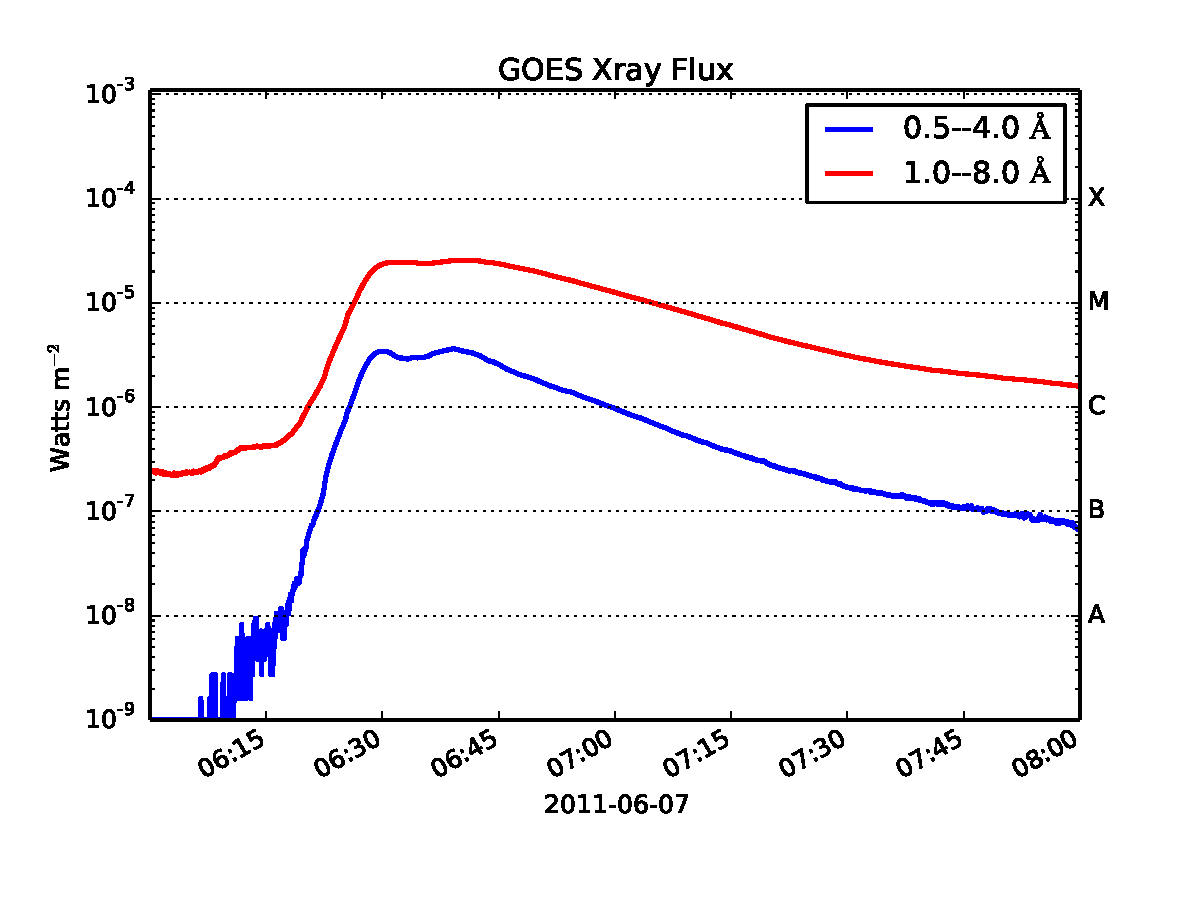
\includegraphics[width=10cm]{goes_lightcurve.pdf}
\end{center}
\caption{Example retrieval of a GOES lightcurve for the time interval 
06:00--08:00 UT on 2011 June 7 using a time range, and the output of the 
\texttt{peek()} method.
Finally the data is resampled to a 1 hour cadence.}
\label{code:goes_lc}
\end{listing}
%schriste - note to self, fix this example, add resampled points on top of plot?

Alternatively, if the data file already exists on the local system, the 
\texttt{Lightcurve} object may instead be initialised using that file as input.
Once the \texttt{Lightcurve} has been created, it may be manipulated in 
a variety of ways in order to perform time-series analysis.

%Stuart: Where did the pandas section go?
